%%
%% This is file `sample-manuscript.tex',
%% generated with the docstrip utility.
%%
%% The original source files were:
%%
%% samples.dtx  (with options: `all,proceedings,bibtex,manuscript')
%% 
%% IMPORTANT NOTICE:
%% 
%% For the copyright see the source file.
%% 
%% Any modified versions of this file must be renamed
%% with new filenames distinct from sample-manuscript.tex.
%% 
%% For distribution of the original source see the terms
%% for copying and modification in the file samples.dtx.
%% 
%% This generated file may be distributed as long as the
%% original source files, as listed above, are part of the
%% same distribution. (The sources need not necessarily be
%% in the same archive or directory.)
%%
%%
%% Commands for TeXCount
%TC:macro \cite [option:text,text]
%TC:macro \citep [option:text,text]
%TC:macro \citet [option:text,text]
%TC:envir table 0 1
%TC:envir table* 0 1
%TC:envir tabular [ignore] word
%TC:envir displaymath 0 word
%TC:envir math 0 word
%TC:envir comment 0 0
%%
%%
%% The first command in your LaTeX source must be the \documentclass
%% command.
%%
%% For submission and review of your manuscript please change the
%% command to \documentclass[manuscript, screen, review]{acmart}.
%%
%% When submitting camera ready or to TAPS, please change the command
%% to \documentclass[sigconf]{acmart} or whichever template is required
%% for your publication.
%%
%%
\documentclass[manuscript,screen,review]{acmart}

\usepackage{caption}
\usepackage[utf8]{inputenc}
\usepackage[capitalize, noabbrev]{cleveref}

%%
%% \BibTeX command to typeset BibTeX logo in the docs
\AtBeginDocument{%
  \providecommand\BibTeX{{%
    Bib\TeX}}}

%% Rights management information.  This information is sent to you
%% when you complete the rights form.  These commands have SAMPLE
%% values in them; it is your responsibility as an author to replace
%% the commands and values with those provided to you when you
%% complete the rights form.
\setcopyright{acmlicensed}
\copyrightyear{2024}
\acmYear{2024}
\acmDOI{XXXXXXX.XXXXXXX}

%% These commands are for a PROCEEDINGS abstract or paper.
\acmConference[Koli Calling '24]{24th Koli Calling International Conference on Computing Education Research}{November 14--17,
  2024}{Koli, Finland}
%%
%%  Uncomment \acmBooktitle if the title of the proceedings is different
%%  from ``Proceedings of ...''!
%%
%%\acmBooktitle{Woodstock '18: ACM Symposium on Neural Gaze Detection,
%%  June 03--05, 2018, Woodstock, NY}
% \acmISBN{978-1-4503-XXXX-X/18/06}


%%
%% Submission ID.
%% Use this when submitting an article to a sponsored event. You'll
%% receive a unique submission ID from the organizers
%% of the event, and this ID should be used as the parameter to this command.
%%\acmSubmissionID{123-A56-BU3}

%%
%% For managing citations, it is recommended to use bibliography
%% files in BibTeX format.
%%
%% You can then either use BibTeX with the ACM-Reference-Format style,
%% or BibLaTeX with the acmnumeric or acmauthoryear sytles, that include
%% support for advanced citation of software artefact from the
%% biblatex-software package, also separately available on CTAN.
%%
%% Look at the sample-*-biblatex.tex files for templates showcasing
%% the biblatex styles.
%%

%%
%% The majority of ACM publications use numbered citations and
%% references.  The command \citestyle{authoryear} switches to the
%% "author year" style.
%%
%% If you are preparing content for an event
%% sponsored by ACM SIGGRAPH, you must use the "author year" style of
%% citations and references.
%% Uncommenting
%% the next command will enable that style.
%%\citestyle{acmauthoryear}


%%
%% end of the preamble, start of the body of the document source.
\begin{document}

%%
%% The "title" command has an optional parameter,
%% allowing the author to define a "short title" to be used in page headers.
% \title{Automated Feedback Loops: Enhancing Student Motivation and Performance in Programming Courses}
\title{Direct automated feedback for student submissions based on LLMs}

%%
%% The "author" command and its associated commands are used to define
%% the authors and their affiliations.
%% Of note is the shared affiliation of the first two authors, and the
%% "authornote" and "authornotemark" commands
%% used to denote shared contribution to the research.


\author{Maximilian Sölch}
\email{maximilian.soelch@tum.de}
\orcid{0009-0004-1509-7842} 
\affiliation{%
	\institution{Technical University of Munich}
	\city{Munich}
	\country{Germany}
}

\author{Felix T.J. Dietrich}
\email{felixtj.dietrich@tum.de}
\orcid{0009-0007-5826-2061} 
\affiliation{%
	\institution{Technical University of Munich}
	\city{Munich}
	\country{Germany}
}

\author{Stephan Krusche}
\email{krusche@tum.de}
\orcid{0000-0002-4552-644X}
\affiliation{%
	\institution{Technical University of Munich}
	\city{Munich}
	\country{Germany}
}

%%
%% By default, the full list of authors will be used in the page
%% headers. Often, this list is too long, and will overlap
%% other information printed in the page headers. This command allows
%% the author to define a more concise list
%% of authors' names for this purpose.
\renewcommand{\shortauthors}{Sölch et al.}

%%
%% The abstract is a short summary of the work to be presented in the
%% article.
\begin{abstract}
  A clear and well-documented \LaTeX\ document is presented as an
  article formatted for publication by ACM in a conference proceedings
  or journal publication. Based on the ``acmart'' document class, this
  article presents and explains many of the common variations, as well
  as many of the formatting elements an author may use in the
  preparation of the documentation of their work.
\end{abstract}

%%
%% The code below is generated by the tool at http://dl.acm.org/ccs.cfm.
%% Please copy and paste the code instead of the example below.
%%
\begin{CCSXML}
  <ccs2012>
     <concept>
         <concept_id>10003456.10003457.10003527.10003540</concept_id>
         <concept_desc>Social and professional topics~Student assessment</concept_desc>
         <concept_significance>500</concept_significance>
         </concept>
     <concept>
         <concept_id>10010405.10010489</concept_id>
         <concept_desc>Applied computing~Education</concept_desc>
         <concept_significance>500</concept_significance>
         </concept>
   </ccs2012>
\end{CCSXML}
  
\ccsdesc[500]{Social and professional topics~Student assessment}
\ccsdesc[500]{Applied computing~Education}

%%
%% Keywords. The author(s) should pick words that accurately describe
%% the work being presented. Separate the keywords with commas.
\keywords{Do, Not, Us, This, Code, Put, the, Correct, Terms, for,
  Your, Paper}

% \received{20 February 2007}
% \received[revised]{12 March 2009}
% \received[accepted]{5 June 2009}

%%
%% This command processes the author and affiliation and title
%% information and builds the first part of the formatted document.
\maketitle

\section{Introduction} % 1 page

% problem
% time consuming, not scalable, not always available
% hinders learning progress and motivation %todo: reference for this!

% todo: reference for this!
In the current educational landscape, providing timely and effective feedback to students remains a significant challenge.
Traditionally, students must wait for course tutors or professors to review their submissions and provide feedback.
This process can be time-consuming, often requiring students to arrange meetings and wait for available time slots, which are not always convenient or immediate.
The inherent delays and scheduling difficulties make this approach not scalable, especially in courses with a large number of students.

% todo: reference for this!
These limitations hinder students' learning progress and motivation.
The waiting period for feedback interrupts the learning flow, causing students to lose momentum and potentially disengage from the subject matter.
%todo: reference for this!
Additionally, the limited availability of tutors and professors means that not all students receive the individualized attention they need to improve their understanding and skills.
This situation underscores the necessity for a more efficient and scalable feedback system that can provide continuous support to students without the constraints of traditional methods.


% Objectives


%Outline
The subsequent sections of this paper are organized to provide a comprehensive understanding of the research. 
\cref{sec:related-work} provides an overview of related work. 
\cref{sec:approach:DAFeeD} details the concept and methodology of Direct Automated Feedback Delivery (DAFeeD).
\cref{sec:reference-implementation} describes the reference implementation of DAFeeD, called Athena, including a general overview, details on the used prompts, and the system architecture. 
\cref{sec:evaluation} presents the evaluation results, %todo: add results 
Finally, \cref{sec:conclusion} concludes with a summary of findings and discusses future research directions to enhance automated feedback systems.

\newpage
\section{Related Work} % 2 page
\label{sec:related-work}
todo
\cite{hahn:2021:SystematicReviewEffects}

\newpage
\section{Approach: Direct Automated Feedback Delivery (DAFeeD)} % 1 page
\label{sec:approach:DAFeeD}

DAFeeD employs large language models to deliver automated feedback on student submissions, designed to complement traditional teaching methods and provide additional support.
Figure \ref{fig:DAFeeD-workflow} illustrates the continuous feedback workflow that DAFeeD facilitates, enabling students to receive feedback at any time, thereby eliminating the need to wait for responses from human tutors or course professors.

\begin{figure}[htbp]
  \centering
  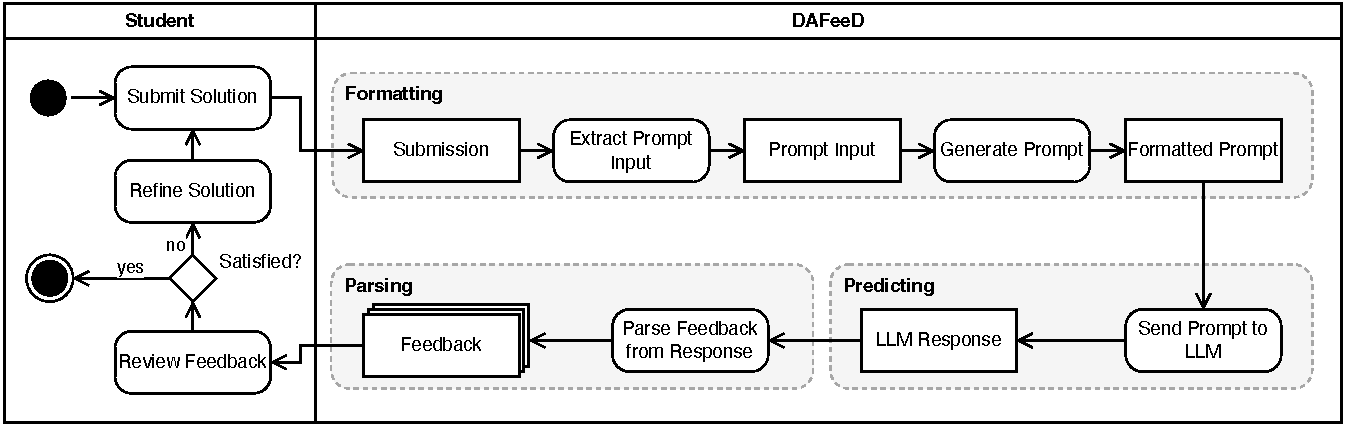
\includegraphics[width=\linewidth]{figures/DAFeeD-ActivityDiagram.pdf}
  \caption{Workflow of direct automated feedback delivery for students' submissions (UML Activity Diagram)}
  \label{fig:DAFeeD-workflow}
\end{figure}

DAFeeD can provide feedback on various aspects, such as the correctness of the code, the quality of the code, and the performance of the student.
Once the student submits their solution, DAFeeD initiates a three-stage process to generate natural language feedback.

The first stage, called \textit{Formatting}, takes the student's submission and extracts the submission content, problem statement including learning objectives, and any possible grading instructions the instructor defines.
This extracted information represents the prompt input.
During the prompt generation step, a predefined prompt template is filled with the prompt input data, resulting in a formatted prompt.

In the second stage, called \textit{Predicting}, the formatted prompt is sent to a large language model, which generates a response that includes detailed feedback for the student.

The final stage, \textit{Parsing}, takes the LLM response, which comes in the JSON format, and parses feedback items from it. 
In addition to the feedback text, the feedback object also contains reference information indicating the part of the submission it pertains to.
For programming exercises, this includes the file name and line number of the relevant code snippet to which the feedback refers.
For text exercises, the reference information includes only the sentence or word range the feedback refers to.

All of the feedback is then returned to the student for review.
If the student is satisfied with the feedback, the process concludes. 
Otherwise, the student can refine their solution and resubmit it, initiating the DAFeeD process anew.

This iterative process is designed to motivate students to continuously learn and experiment with their solutions, resulting in improved performance.


\section{Reference Implementation: Athena} % 2 pages
\label{sec:reference-implementation}

We incorporated DAFeeD into a reference implementation named Athena, which is integrated with the learning platform Artemis through which students submit their solution and review the feedback.


%todo: visualization of the feedback in Artemis

\subsection{Prompts}

%Todo: Listing of the used prompt (at least simplified) and an explanation of the prompt

\subsection{Feedback Generation}
?

\subsection{Architecture}
%Todo: deployment diagram + description
Modular approach to support multiple exercise types and extend it in the future

The assessment module manager receives all requests, checks for authorization, and then forwards them to the responsible modules.

Independent of a specific learning management system, provides a REST API documented with the OpenAPI standard

Currently connected to OpenAI and Azure OpenAI 
Can be simply modified to use open-source models like Llama or Mistral either self-hosted or in the cloud.


As the reference implementation is used in conjuction with the Artemis learning management system for actual university courses, the system is designed to be scalable and reliable (performance, maintainability, usability)
Deployed in a kubernetes cluster to ensure scalability and reliability, loadbalancing, etc.
Scale each module independently, e.g., more instances of the programming module when a new programming exercise is released.

\section{Evaluation} % 5 pages
\label{sec:evaluation}

\subsection{Research Questions}

\subsection{Study Design}

\subsection{Results}

\subsection{Limitations}

\subsection{Discussion}


\section{Conclusion \& Future Work} % 1 page
\label{sec:conclusion}

%future work
% 
Future work includes enhancing the visualization of feedback, such as grouping and color coding the feedback items to make it easier to differentiate between critical feedback items, suggestions for improvement, and positive feedback.
A high priority will be on further improving the overall quality of the feedback provided. 
We also aim to extend the implementation to support direct automated feedback for the remaining exercise types of Artemis.
Another crucial step is to test direct automated feedback in a real-world setting by utilizing this feature in an actual course. 
This will allow us to collect comprehensive data to thoroughly evaluate the impact on student performance and motivation.


%%
%% The next two lines define the bibliography style to be used, and
%% the bibliography file.
\bibliographystyle{ACM-Reference-Format}
\bibliography{main}

\end{document}
\endinput
%%